\documentclass[12pt, landscape]{article}
\usepackage[scaled=0.92]{helvet}
\usepackage{multicol}
\usepackage{calc}
\usepackage{ifthen}
\usepackage[landscape]{geometry}
%\usepackage{hyperref}

\usepackage{newtxtext} 

%for strikeout
\usepackage{ulem}

%For editing parbox
\usepackage[table]{xcolor}
%For editing itemise margins, reduce item separaion and list separation
\usepackage{enumitem}
\setlist[itemize]{noitemsep}

% For math
\usepackage{amsmath,amsthm,amsfonts,amssymb}

% For justifying
\usepackage{ragged2e}
\justifying

%For pictures / figures
\usepackage{color,graphicx,overpic}
\graphicspath{ {./images/} }

%\usepackage{newtxtext} 
%\usepackage{amssymb}
%\usepackage[table]{xcolor}
%\usepackage{vwcol}
%\usepackage{tikz}
%\usepackage{wrapfig}
%\usepackage{makecell}


% For Code Blocks
\usepackage{xcolor}
\usepackage{listings}

\lstdefinestyle{mystyle}{
	backgroundcolor=\color{gray!25!white},
	basicstyle=\scriptsize,
	numbers=none,    %or = none or left
	showstringspaces=false,
	breaklines=true,
	breakatwhitespace=false,                  
	captionpos=b,                    
	keepspaces=true,                                 
	numbersep=3pt,                  
	showspaces=false,                
	showtabs=false,                  
	tabsize=2,
 }


%Helpful:
%[linewidth = 1.0 \linewidth]
%\lstinline{}
% use \code{} for \lstinline with colorbox.
\newcommand{\code}[1]{\colorbox{gray!25!}{\lstinline|#1|}}
\lstset{style=mystyle}

% Template: Cheatsheet with code enabled

%--------------------------- PACKAGES ABOVE --------------------------------------------------------------

\pdfinfo{
  /Title (Documentname.pdf)
  /Creator (Ger Teck)
  /Author (Ger Teck)
  /Subject ()
  /Keywords (tex)}

%% Margins for PAPER

% This sets page margins to .5 inch if using letter paper, and to 1cm
% if using A4 paper. (This probably isn't strictly necessary.)
% If using another size paper, use default 1cm margins.
\ifthenelse{\lengthtest { \paperwidth = 11in}}
	{ \geometry{top=.5in,left=.5in,right=.5in,bottom=.5in} }
	{\ifthenelse{ \lengthtest{ \paperwidth = 297mm}}
		{\geometry{top=1cm,left=1cm,right=1cm,bottom=1cm} }
		{\geometry{top=1cm,left=1cm,right=1cm,bottom=1cm} }
	}

% Turn off header and footer
\pagestyle{empty}

% for tight centres (less spacing)
\newenvironment{tightcenter}{%
  \setlength\topsep{0.5pt}
  \setlength\parskip{0.5pt}
  \begin{center}
}{%
  \end{center}
}

% Redefine section commands to use less space
\makeatletter
\renewcommand{\section}{\@startsection{section}{1}{0mm}%
                                {-1ex plus -.5ex minus -.2ex}%
                                {0.5ex plus .2ex}%x
                                {\normalfont\large\bfseries}}
\renewcommand{\subsection}{\@startsection{subsection}{2}{0.1mm}%
                                {-1explus -.5ex minus -.2ex}%
                                {0.5ex plus .2ex}%
                                {\normalfont\normalsize\bfseries}}
\renewcommand{\subsubsection}{\@startsection{subsubsection}{3}{0.1mm}%
                                {-1ex plus -.5ex minus -.2ex}%
                                {1ex plus .2ex}%
                                {\normalfont\small\bfseries}}
% change font
%\renewcommand{\familydefault}{\sfdefault}
%\renewcommand\rmdefault{\sfdefault}
\linespread{1.05}

\makeatother

% Define BibTeX command
\def\BibTeX{{\rm B\kern-.05em{\sc i\kern-.025em b}\kern-.08em
    T\kern-.1667em\lower.7ex\hbox{E}\kern-.125emX}}

% Don't print section numbers
\setcounter{secnumdepth}{0}

\setlength{\parindent}{0pt}
\setlength{\parskip}{0pt plus 0.5ex}

%% this changes all items (enumerate and itemize, reduce margins)
\setlength{\leftmargini}{0.5cm}
\setlength{\leftmarginii}{0.5cm}
\setlist[itemize,1]{leftmargin=2mm,labelindent=1mm,labelsep=1mm, itemsep = 1mm}
\setlist[itemize,2]{leftmargin=4mm,labelindent=1mm,labelsep=1mm, itemsep = 1mm}
%itemsep = 0mm
%\setlist{nosep}

% Need Logo Picture
%Watermark Top Right
%\usepackage{atbegshi,picture}
%\AtBeginShipout{\AtBeginShipoutUpperLeft{%
 % \put(\dimexpr\paperwidth-1.2cm\relax, -1.2cm){\makebox[0pt][r]{\framebox{
\includegraphics[width = 0.3cm]{mountainbooks} Ger Teck}}}%
%}}


% -------------------------------------------------------------------------------

% START OF DOCUMENT HERE

\begin{document}
\raggedright
\footnotesize
\begin{multicols*}{3}



% multicol parameters
% These lengths are set only within the two main columns
%\setlength{\columnseprule}{0.25pt}
\setlength{\premulticols}{1pt}
\setlength{\postmulticols}{1pt}
\setlength{\multicolsep}{1pt}
\setlength{\columnsep}{2pt}

%% DOCUMENT NAME HERE
\begin{center}
     \Large{\textbf{CS2102 Database Sys Summary}} \\
\end{center}

AY23/24 Sem 1, github.com/gerteck
  
\section{Topics \& Objectives}
\justify{
\begin{itemize}
	\item \textbf{Design}: Entity-Relationship (ER) Model, Functional Dependencies, Normal Forms
	\item \textbf{Implementation}: SQL (Data definition language, Queries, Stored procedures, Triggers)
	\item\textbf{Theory}: Relational Calculus and algebra
	\item Module covers fundamental concpets and techniques for:
	\begin{itemize}
		\item Understanding and practice of design \& implementation of database applications and management of data with relational db management systems.
		\item Design of ER data models to capture data requirements, translate to relational database schema, refine using schema decompositions to avoid anomalies.
		\item Use SQL to define relational schemas, write queries.
		\item Reason about correctness using concepts of formal query lang (relational calculus \& algebra) and apply knowledge to develop database applications.	
	\end{itemize}
\end{itemize}
}
\centerline{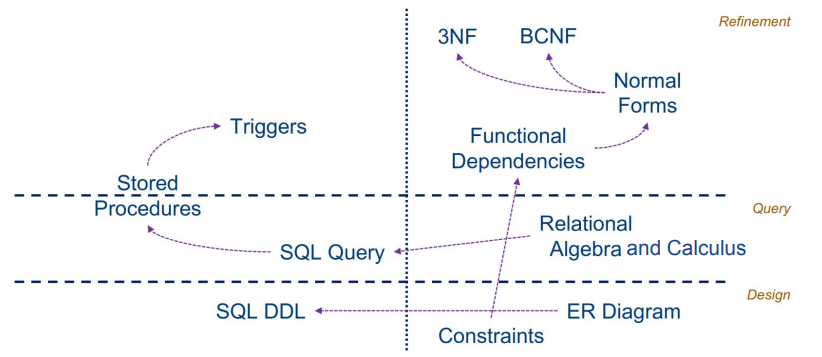
\includegraphics[width=0.9 \linewidth]{roadmap}}

\section{1. Database Management Sys DBMS}
\subsubsection{Challenges for Data-Intensive applications}
\justify{
\begin{itemize}
	\item \textbf{Efficiency}: Fast access to information in volumes of data
	\item \textbf{Transactions}: "All or nothing" changes to data
	\item \textbf{Data Integrity}: Parallel access and changes to data
	\item \textbf{Recovery}: Fast and reliable handling of failures (e.g. HDD/Sys crash, power outage, network disruption)
	\item \textbf{Security}:  Fine-grained data access rights
\end{itemize}
  
\subsubsection{File-based data management to DBMS}
\begin{itemize}
	\item Complex, low level code, Often similar requirements across different programs
	\item \textbf{Problems}:  High development effort, Long development times, Higher risk of (critical) errors
	\item \textbf{DBMS}:  Set off universal and powerful functionalities for data management, with faster application development, higher stability, less errors.
\end{itemize}

\subsubsection{Core concepts of DBMS}
\begin{itemize}
	\item \textbf{ACID Transaction}:  Finite sequence of database operations (reads and/or writes), smallest logical unit of work
	\item \textbf{Atomicity}:  either all effects of T are reflected in the database or none ("all or nothing")
	\item \textbf{Consistency}: the execution of T guarantees to yield a correct state of the database
	\item \textbf{Isolation}:  execution of T is isolated from the effects of concurrent transactions
	\item \textbf{Durability}: after commit of T, its effects are permanent even in case of failures 
\end{itemize}

\subsubsection{Concurrent Execution}
\centerline{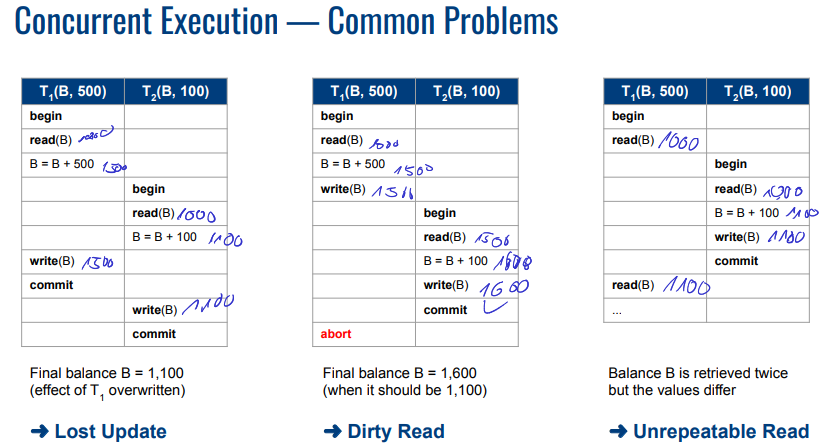
\includegraphics[width=0.7 \linewidth]{concurrentproblems}}
Require Serializable transaction execution:
\begin{itemize}
	\item A concurrent execution of a set of transactions is serializable if this execution 
	is equivalent to some serial execution of the same set of transactions
	\item Two executions are equivalent if they have the same effect on the data
	\item \textbf{DBMS}: Support concurrent executions of transactions to optimize performance, Enforce serializability of concurrent executions to ensure integrity of data
\end{itemize}
}

\subsubsection{Data Abstraction}
\centerline{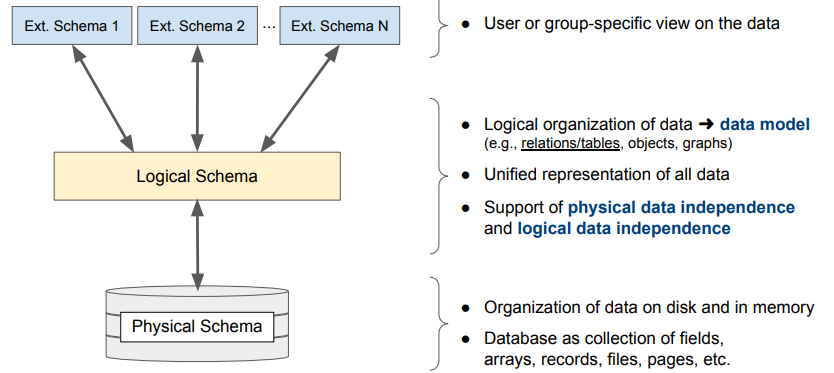
\includegraphics[width=0.9 \linewidth]{dataabstraction}}
\subsubsection{Data Independence}
\centerline{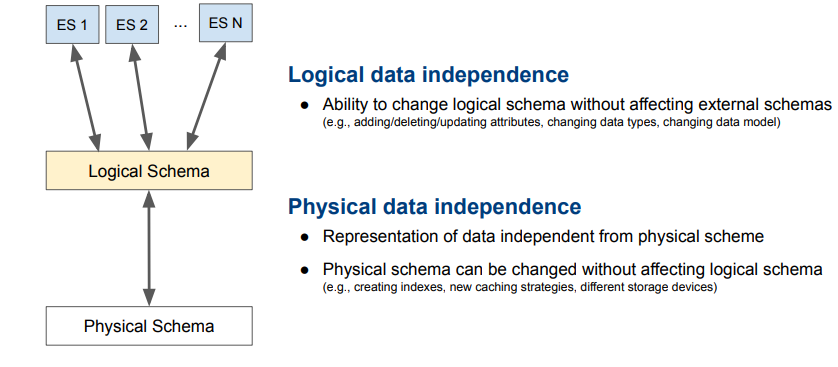
\includegraphics[width=0.9 \linewidth]{dataindependence}}

\justify{
\subsection{Terminology / Definitions}
\begin{itemize}
	\item \textbf{Data Model}: Collection of concepts for describing data
	\item \textbf{Schema}: Description of structure of DB using data model
	\item \textbf{Schema Instance}: Content of a DB at a particular time
\end{itemize}
\subsubsection{Relational Data Model}
Data is modelled by relations, and each relation has a definition called a relation schema. This schema specifies attributes (columns) and data constrains (e.g. domain constraints)
\begin{itemize}
	\item \textbf{Relation}: Can be seen as Tables with rows and columns:
	\begin{itemize}
		\item No. of cols = Degree/Arity, No. of rows = Cardinality
		\item Each row is called a tuple/record. It has a component for each attribute of the relation.
		\item A relation is thus a set of tuples and an instance of the relation schema, i.e. of a single table.
	\end{itemize}
	\item \textbf{Domain}: Set of atomic values, e.g. integers. All values for an attribute is either in this domain or null.
	\item \textbf{Relational database schema}: Set of relation schemas and their data constraints, i.e. of multiple tables
	\item \textbf{Relational database}:  Instance of the schema and is a collection of tables.
\end{itemize}
\centerline{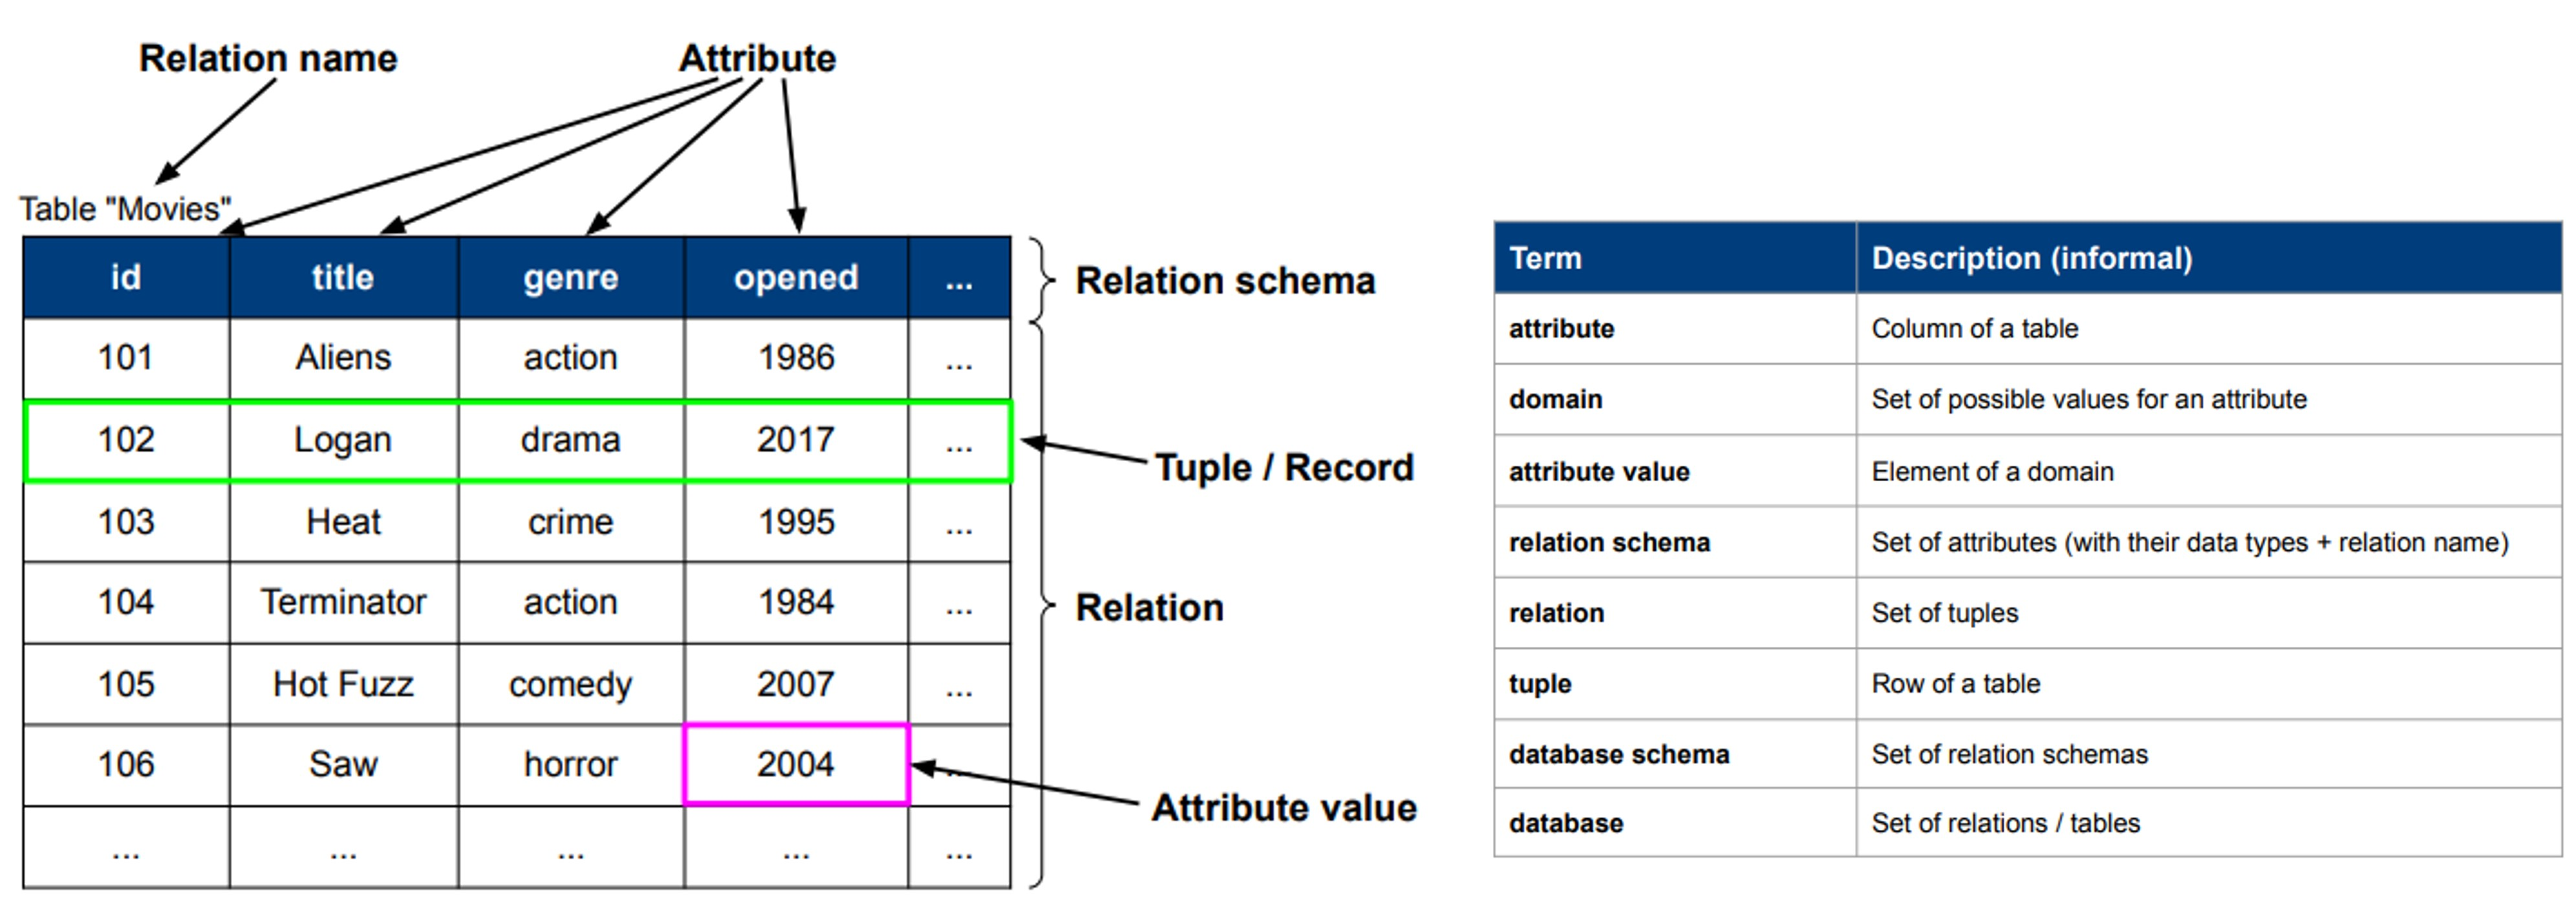
\includegraphics[width=1 \linewidth]{relationalterms}}

\subsection{Integrity Constraints}
Condition that restricts the data that can be stored in a database instance. A legal relation instance is a relation that satisfies all specified ICs.
\begin{itemize}
	\item \textbf{Domain Constraints}:  Restrict the attribute values of relations, e.g. only integers allowed
	\item \textbf{Key Constraints}:
	\begin{itemize}
		\item \textbf{Superkey}: A superkey is a subset of attributes in a relation that unique identifies its tuples.
		\item \textbf{Key}:  A key is a superkey which is minimal, i.e. no proper subset of itself is a superkey. 
		\item \textbf{Candidate keys}: Set of all possible keys for a relation. One of these keys is selected as the primary key.
		\item \textbf{Primary key}: Chosen candidate key for a relation, Cannot be null (entity integrity constraint), Underlined in relation schema. Prime attribute: Attribute of a primary key (cannot be null)
	\end{itemize}
	\item \textbf{Foreign Key Constraints}:
	\begin{itemize}
		\item \textbf{Foreign key}:   A foreign key refers to the primary key of a second relation (which can be itself)
		\item Each foreign key value must be the primary key value in the referenced relation or be null (foreign key constraint)
		\item  Also known as referential integrity constraints.
	\end{itemize}
\end{itemize}
\centerline{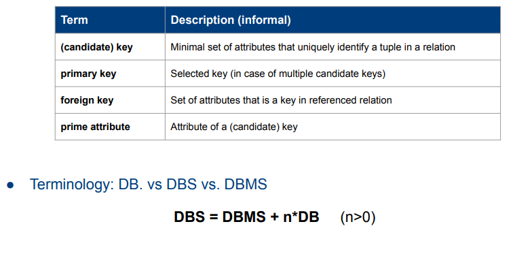
\includegraphics[width=0.8 \linewidth]{integrityconstraints}}
}


























  
  
  
  
\end{multicols*}
\end{document}